\subsection{Climate change and geoengineering}
In the effort of limiting the effects global climate change, eliminating fossil fuels is the most important step to take. Regrettably, the complete elimination of fossil fuels in time to prevent the most disastrous effects of climate change and limit global warming to even 2°C is becoming increasingly unlikely. Even with all currently committed climate action goals, projections show the earth warming significantly above the 1.5°C and 2°C targets from the Paris Agreement \parencite{NDCsynth}. With this outlook, methods to temporarily lower the earth's global temperature are looked at to buy the global community time to lower atmospheric greenhouse gases. One such method is solar radiation management with stratospheric aerosol injections (SAI). 

Geoengineering can be seen as a toolbox of methods that change the earth's climate system to achieve a desired effect. Limiting global mean surface temperature (GMST) increase is the primary goal of geoengineering. The methods of geoengineering can be divided into two basic categories, Carbon Dioxide Removal (CDR) and Solar Radiation Management (SRM) \parencite{shepherd2009}. CDR focuses on lowering the amount of greenhouse gases in the atmosphere, by capturing CO$_2$ directly or enhancing and facilitating natural processes to speed up the extraction of CO$_2$ from the atmosphere or oceans. SRM on the other hand focuses on altering the earth's radiation budget. This can be done by increasing the amount of long wave radiation the earth emits into space, for instance with cirrus cloud thinning, but the most widely discussed approach is increasing how much short wave radiation from the sun is reflected back into space, i.e. increasing the planetary albedo. This is done for instance by making deserts more reflective or making clouds brighter like through marine cloud brightening \parencite{reflecting}. 

\subsection{Geoengineering in the Form of Stratospheric Aerosol Injections}
This thesis considers SRM in the form of stratospheric aerosol injections (SAI). Through injection of sulphate aerosols or their precursors at specific points in the stratosphere the earth's radiation budget is changed. At this high altitude the aerosols reflect short wave radiation, lowering the amount of sunlight reaching the earth's surface and subsequently GMST is lowered. It has been argued that SAI is one of the most feasible options for SRM \parencite{lenton2009,shepherd2009}.

A direct result of SAI is the absorption of long wave radiation emitted by the earth by the aerosols, resulting in warming in the stratosphere \parencite{Ammann2010}. This impacts the global atmospheric circulation patterns and precipitation patterns. It is also important to keep in mind that the effects other than warming caused by increased greenhouse gases are still present in the earth system, for instance ocean acidification will continue if CO$_2$ concentrations continue to rise. The introduction of sulphate aerosols has unintended consequences too, including in delayed repair of the ozone hole and an increase in acid deposition, and interference with cloud formation. 

Eventhough complete understanding of the physical consequences of SAI is not within reach as of now, the physical feasibility in regards to limiting global warming is rather certain. Practically, the succesful deployment of SAI is only possible if the global community can reach consensus on its employment and can ensure no party deploys SAI undemocratically and to the detriment of others. Even then, long-term political and economical stability are crucial, as an abrupt halt would lead to rapid warming \parencite{robock2009}. 

The employment of SAI is not as straight-forward as appears at first glance, and before any decisions can be made about SRM, with SAI or through other means, more research is needed. The National Academy of Sciences made extensive recommendations for solar geoengineering research \parencite{reflecting}, including research into the impacts on atmospheric processes, the climate response, desigining a monitoring system, how to govern solar geoengineering activities and ethical considerations for current and future generations. 

\subsection{General Structure}
In this thesis we investigate the climate response to SAI, more specifically the atmospheric dynamics of the Southern Hemisphere. We will use the results from a previous study on SAI conducted with an earth system model with an extensive atmospheric component and comprehensive atmospheric chemistry to build an emulator with a model with a smaller atmospheric component that incorporates no atmospheric chemistry. We do this primarily to save on computation time. We will validate this experiment in Part I, and use it to assess the impact of SAI on the Southern Hemisphere atmospheric circulation in Part II. We will focus on changes in the large scale components of the atmospheric circulation. 

The southern hemisphere is of particular interest because of the Antarctic Ice Sheet that is home to a number of tipping points. The triggering of these tipping points can potentially lead to disastrous levels of sea level rise and once these tipping points are reached, there is no way to reverse the effects. Understanding the dynamics of the Southern Hemisphere and the response to SAI is crucial to accurately predict the future evolution of these tipping points and if triggering them can be avoided with the help of SAI. 

\newpage
\section{Introduction Part I}
\subsection{Previous Research on SAI in Earth System Models}
Large scale studies on SRM started with the Geoengineering Model Intercomparison Project (GeoMIP) \parencite{geomip2011}. Experiments reduced the incoming solar radiation either directly or through injection of SO$_2$ in the stratosphere at one point on the equator, which was then distributed in the atmosphere very quickly by the zonal circulation and on larger time scales the meridional circulation.

It was found that injection of aerosols at just the equator, and uniform solar radiation reduction lead to over-cooling of the tropics and under-cooling of the poles. \textcite{kravitz2016} proposed a different approach, where climate targets were considered the main goal and how to reach those goals through SAI was viewed as a design problem. One set of targets proposed was the global mean surface temperature ($T_0$), the interhemispheric temperature gradient ($T_1$) and the pole-to-equator temperature gradient ($T_2$). The proposed SAI strategy included four injection points, two on each hemisphere, and a feedback algorithm that adjusts the injection rate at those points to achieve the temperature goals. This method was applied by \textcite{kravitz2017} and \textcite{macmartin2017}, and then in the Geoengineering Large Ensemble (GLENS) project \parencite{tilmes2018}. 

\subsection{The GLENS Project and Subsequent CESM2 Simulations}
The GLENS project is a 20-member ensemble of gradual SAI simulations. From 2020 onwards SO$_2$ is injected at four injection points at $\pm$ 15°N and $\pm$ 30°N about 5 km above the tropopause. A feedback-control algorithm is used to adjust the injection amounts at each point individually based on the departure of the $T_{0,1,2}$ temperatures defined by \textcite{kravitz2016} from 2020 levels.

The GLENS project was performed using the Community Earth System Model version 1 (CESM1) \parencite{hurrell2013}, with the Whole Atmosphere Community Climate Model (WACCM) as its atmosphere component. This model uses a 0.9° latitude $\times$ 1.25° longitude rectangular grid with 70 vertical layers that reach up to 140 km, or about 10$^{-6}$ hPa. It includes comprehensive atmospheric chemistry for the middle atmosphere, incorporating ozone chemistry and chemistry relating to stratospheric sulfate formation. A simpler chemistry scheme is used for the troposphere. Aerosol chemistry is coupled to WACCM through the three-mode version of the Modal Aerosol Module (MAM3).

After the GLENS project the method using four injection points and a feedback algorithm was further explored using the more recent Community Earth System Model version 2, also using a newer version of the WACCM, now version 6 (CESM2(WACCM6)) \parencite{tilmes2020}. WACCM6 has the same horizontal and vertical resolution, but now includes comprehensive chemistry from the troposphere up to the lower thermosphere. The MAM4 modal aerosol scheme is used for the troposphere and stratosphere. We will refer to this model as `WACCM'.

Because WACCM is comprehensive in both vertical resolution and atmospheric chemistry, it is well-suited to simulate SAI scenarios. However, due to this it is also a very cumbersome model, requiring more computing time and resources compared to less comprehensive models. This limits its use in ensemble studies and studies considering a large range of scenarios. Computational cost also limits its use for simulations with a longer timeseries at higher resolution, required to study smaller scale phenomena like tropical cyclones. 

\subsection{Building an Emulator for SAI with CESM2(CAM6)}
Reducing the amount of computing resources needed for an experiment can be done by using a smaller, less comprehensive model and using previous results from WACCM as external forcing to the model, essentially building an emulator. \textcite{pfluger2024} introduce a method for building such an emulator of WACCM to model SAI. They use the same CESM2 model configuration is used as in \textcite{tilmes2020}, but the Community Atmosphere Model version 6 (CAM6) is used for the atmosphere component \parencite{danabasoglu2020}. This model has only 32 vertical levels and no atmospheric chemistry. We will refer to this model as `CAM'. The aerosol field established in the WACCM simulation is used as an external forcing. To maintain 2020 levels of GMST, the necessary globally averaged aerosol optical depth (AOD) field is found though the same feedforward-feedback algorithm. All other forcing fields are then scaled accordingly. In contrast to the WACCM simulations, the temperature gradients $T_1$ and $T_2$ are not adjusted for. 

The WACCM SAI experiment is well-suited to build an emulator for, as the employment of SAI is used as a means to reach a climatic goal. It prescribes an aerosol burden in response to model behaviour, in stead of gauging the model response to a certain aerosol burden. This removes the amount of SO$_2$ injected into the stratosphere from the experiment design and allows for translation of the aerosol distribution to another model that might respond differently to the introduction of aerosols.

\subsection{Scenarios Part I}
There are two simulations performed with CAM and WACCM. The first simulation follows the historical spin-up and is continued by the SSP5-8.5 scenario \parencite{RIAHI2007887}. The second simulation branches from the first simulation in 2020 and from then on introduces SAI to stabilise temperatures using the SSP5-8.5 scenario as background. Here we will refer to it as the gradual SAI scenario. A schematic view of the GMST response in each scenario is shown in Figure \ref{fig:schematic_scens_pt1}.

\begin{figure}[H]
    \centering
    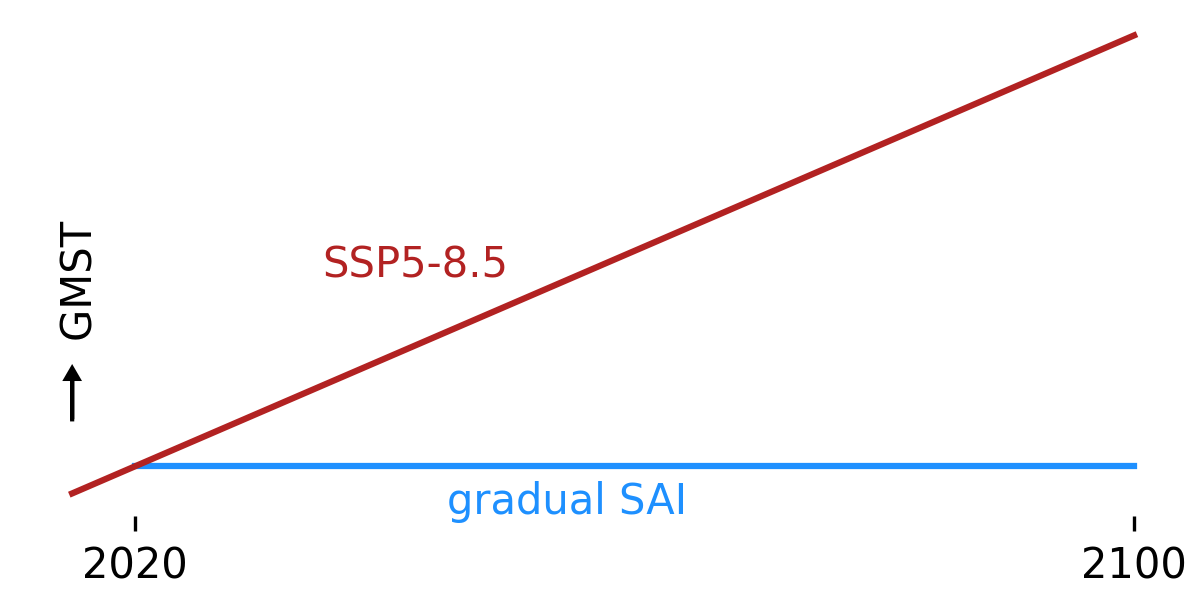
\includegraphics[width=0.6\linewidth]{images/schematic_scens_pt1.png}
    \caption{Schematic of the global mean surface temperature in the two scenarios used in Part I, the SSP5-8.5 and gradual SAI scenarios.}    
    \label{fig:schematic_scens_pt1}
\end{figure}


\newpage
\subsection{Research Questions Part I}
The fist part of this thesis is the validation of this method and model in its use as an emulator, simulating SAI scenarios based on the WACCM results. Two experiments, a high-warming scenario and a gradual SAI scenario, are used to assess the impact of SAI in each model (CAM and WACCM). We calculate the three temperature targets for all models and we will look at the model results for 2-meter temperature for additional insight into the performance of CAM in regards to regulating surface temperatures. We discuss both annual and seasonal patterns. Additionally, we discuss precipitation patterns.

The most important difference in dynamics between the two models lies in the inclusion of ozone chemistry and thus the interaction of stratospheric aerosols and ozone. It is known that sulphate aerosols in the stratosphere accelerate chemical ozone loss through halogen activation and strengthening of the polar vortex \parencite{bednarz2023ozone}. CAM does not include this process, and assessing whether the dynamical response to SAI is comparable to WACCM is thus important. To this end we assess any differences in the vertical profile between the two models, we compare the zonally averaged potential temperature and zonal winds. 

We formulate the following research questions for Part I:
\newline

\noindent \textit{When applying the stratospheric aerosol emulator to a gradual SAI scenario in CESM2(CAM6), are we able to reproduce from \textcite{tilmes2020}
    \begin{enumerate}[label=\roman*]
        \item the temperature targets $T_0$, $T_1$ and $T_2$?
        \item the spatial and seasonal variations of temperature, precipitation and general aspects of the atmospheric circulation?
    \end{enumerate}
}

\subsection{Results SAI in WACCM}
The experiments performed with WACCM \parencite{tilmes2020} showed that surface temperatures were generally controlled with SAI. Under SAI the tropics warmed slightly, the mid-latitudes cooled slightly and the poles warmed slightly as well. Zonal mean precipitation showed an increase in the tropics and a decrease or no significant change everywhere else. An apparent warming hole over the Northern Atlantic was observed in all simulations and was likely related to observed changes in the Atlantic Meridional Overturning Circulation. No changes in seasonal patterns were discussed, nor were changes in potential temperature and atmospheric circulation. 


\newpage
\section{Introduction Part II}
\subsection{Rapid Cooling with SAI as an Emeregency Intervention}
As sufficient climate policies to prevent global warming of 1.5°C or even 2°C \parencite{NDCsynth}, it is unlikely the global community will implement a proactive gradual SAI scenario in time as well. Employing SAI much later on after prolonged heating of the climate system is a realistic, more reactive, scenario. The earth could be cooled very rapidly, allowing the end-of-century GMST goals to be reached after the climate system has endured an even longer period of warming than it has to date. The effects of such an intervention are largely uncertain. While it is rather certain that SAI could lower GMST, it is not certain what effects of previous warming can be reversed, if at all. The SAI 2080 scenario introduced in \textcite{pfluger2024} is such a scenario, SAI is employed from 2080 onwards to achieve rapid cooling to 2020 levels. 

\subsection{Scenarios Part II}
For the second part of this thesis we consider the two CAM simulations from Part I, the SSP5-8.5 and the gradual SAI simulations, and the SAI 2080 scenario from \textcite{pfluger2024}. We will refer to this simulation as the rapid cooling SAI simulation. The rapid cooling simulation is branched from the SSP5-8.5 simulation in 2080, SAI is then deployed to restore $T_0$ to 2020 levels. The control algorithm is adjusted up to the first six years to prevent extremely high aerosol concentrations that would result in too rapid cooling. A schematic view of the GMST response for this scenario is shown in Figure \ref{fig:schematic_scens}.

\begin{figure}[H]
    \centering
    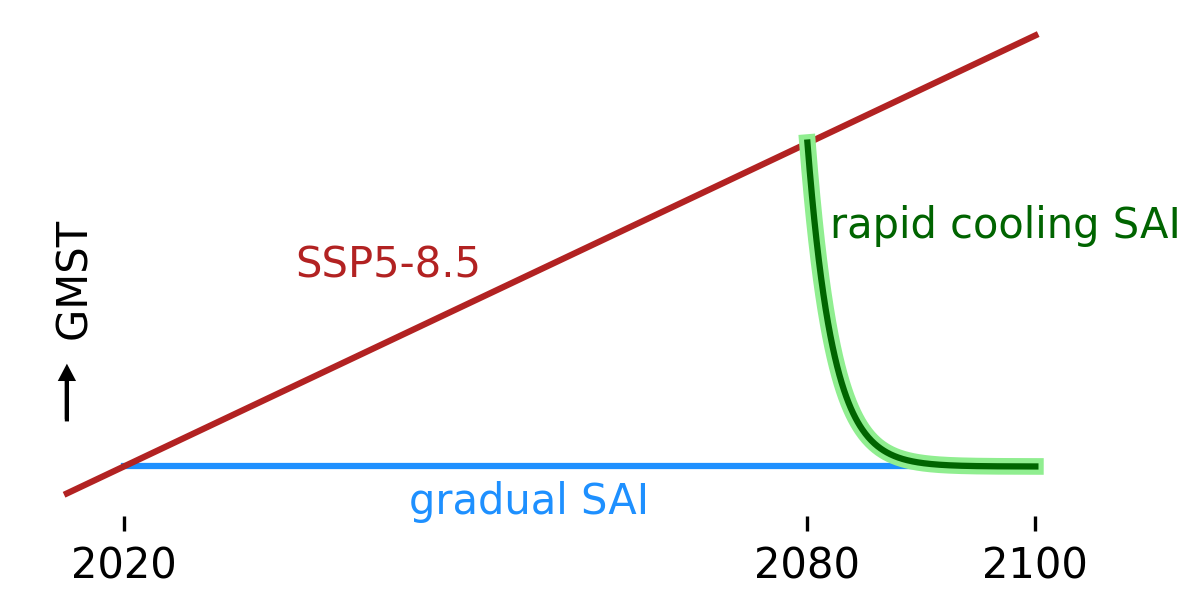
\includegraphics[width=0.65\linewidth]{images/schematic_scens.png}
    \caption{Schematic of the global mean surface temperature in the two scenarios used in Part I, the SSP5-8.5, the gradual SAI and the rapid cooling SAI scenarios.}  
    \label{fig:schematic_scens}  
\end{figure}


\subsection{The Southern Hemisphere Atmopshere}
The atmosphere is home to a number of large scale circulation phenomena. Though the two hemispheres are symmetrical in the occurence of these phenomena, the exact location, frequency of occurence and other behaviour of these phenomena differs between the two hemispheres. The Southern Hemisphere circulation is generally more stable than its counterpart in the Northern Hemisphere. In this thesis we focus on three so-called jets, large scale circulation phenomena that persist throughout the year or in a specific season.
We discuss the subtropical jet and the the eddy-driven jet in the lower stratosphere (up to 50 hPa), and the polar night jet in the upper stratosphere (above 50 hPa).


\subsubsection{The Subtropical Jet}
The subtropical jet (STJ) forms at the convergence of the upper branches of the Hadley and Ferrel cells in the lower stratosphere, with a maximum around 200 hPa, see Figure \ref{fig:jetcrosssection} (the Southern Hemisphere is analogous to the Northern Hemisphere). Influenced by the Coriolis force westerly winds form here, the magnitude of which is determined by the temperature gradient below the convergence zone \parencite{zolotov2018variability}. The STJ occurs year-round but is strongest in winter, in tandem with the stronger winter Hadley cell, where it is located around 30°S.

In the past decades, the southern hemisphere STJ has been observed to shift poleward and slightly decrease in wind speed, though not significant \parencite{zolotov2018variability}. The STJ was also observed to be increasingly wavy \parencite{martin2023}. Under high global warming the STJ is projected to shift further poleward and increase in strength \parencite{chenoli2017historical}. 

Simulations with SAI at singular injection points showed a small but significant decrease in the strength of the STJ \parencite{richter2017}. From historical simulations it has been argued as well that anthropogenic aerosols contribute to deceleration \parencite{wang2020}.

\begin{figure}[t]
    \centering
    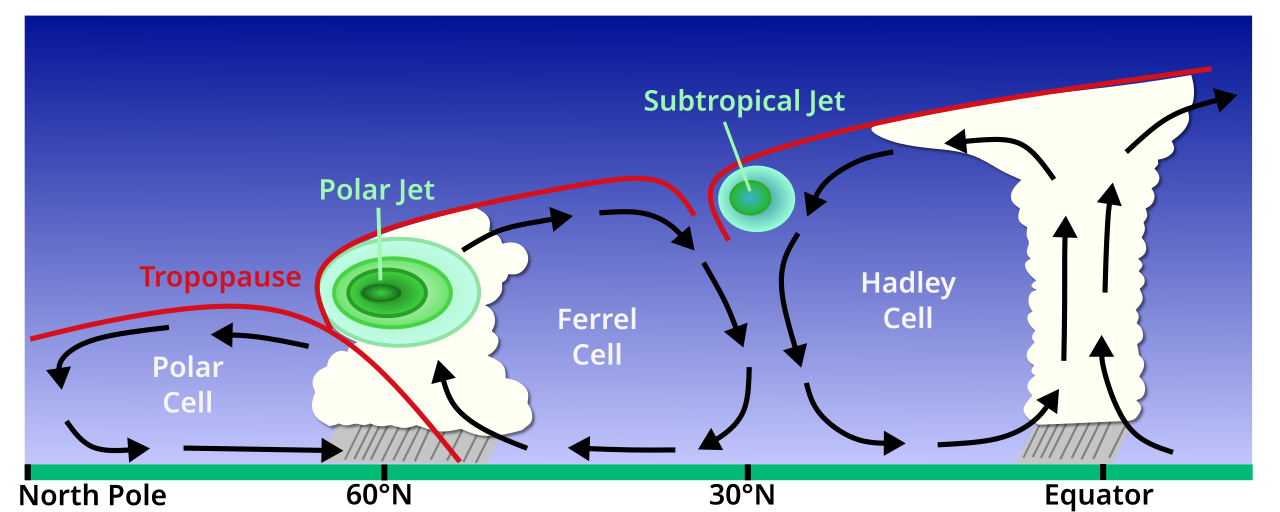
\includegraphics[width=0.8\linewidth]{images/Jetcrosssection.png}
    \caption{Cross section of the Northern Hemisphere atmospheric ciruclation, with the suptropical jet and polar jet (or eddy-driven jet) in relation to the circulation cells. Image by: Original: National Weather Service, JetStream Vector: Sleske - Own work based on: Jetcrosssection.jpg, CC BY-SA 4.0, \href{https://commons.wikimedia.org/w/index.php?curid=75169357}{https://commons.wikimedia.org/w/index.php?curid=75169357}}  
    \label{fig:jetcrosssection}  
\end{figure}


\subsubsection{The Eddy-driven Jet}
At the divergence of the upper branches of the Ferrel and Polar cells another jet forms, the polar jet in Figure \ref{fig:jetcrosssection}. This jet is at a lower altitude and stronger than the STJ. However, it is also much wavier than the STJ \parencite{martin2023}. Because of this, and to avoid confusion with the polar night jet, we will refer to this jet as the eddy-driven jet (EDJ). 

The EDJ has been observed to become increasingly wavy in the past decades, also shifting poleward, even more strongly than the STJ, but no significant trend in the wind speed was observed \parencite{martin2023}. Under high global warming the EDJ is projected to shift further poleward \parencite{Curtis_2020}.

It is not certain how the EDJ will respond under SAI, though it has been shown that the EDJ is influenced by the strength of the polar night jet in the upper stratosphere, where a strengthened jet leads to a poleward shift of the EDJ \parencite{kidston2015stratospheric}. Any changes in the polar night jet due to SAI are thus likely to cause changes in the EDJ as well.

\subsubsection{The Polar Night Jet}
The polar night jet (PNJ) forms in the upper stratosphere during winter in response to the large equator-to-pole meridional temperature gradient. The pole becomes encircled with a belt of strong westerly winds in the upper parts of the stratosphere, above $\approx$50 hPa at around 60°S \parencite{lee2021}. 

With high warming the PNJ is projected to increase in strength, most notably in late SH spring, effectively delaying the ultimate breakdown of the PNJ \parencite{ceppi2019}.

The warming in the lower stratosphere due to SAI leads to an increase of the equator-to-pole meridional temperature gradient, causing increasing zonal winds via the thermal wind balance. This effect is strongest in the late winter/early spring \parencite{bednarz2023injection,bednarz2023ozone}.

When disturbances near the surface propagate to the stratosphere, the PNJ can suddenly weaken, leading to a sudden increase in temperatures of the polar stratosphere and sometimes a complete breakdown of the jet. These events are called sudden stratospheric warming events (SSWs) and occur very rarely in the Southern Hemisphere in the current climate. Their frequency is projected to strongly decrease with increasing global warming \parencite{jucker2021}. 


\subsection{Antarctica and the Southern Hemisphere Atmosphere}
The high-latitude Southern Hemisphere is of particular interest in the context of climate change and the prevention of it. The Antarctic Ice Sheet (AIS) could contribute greatly to global sea level rise if it were to become unstable under global warming. Observed instabilities of the West-Antarctic Ice Sheet (WAIS) alone could contribute to significant sea level rise \parencite{IPCC_2021_WGI_Ch_9}. 

Large scale atmospheric dynamical changes affect the Antarctic ice sheet, changes in temperature, precipitation and wind fields alter the surface mass balance of the ice sheet. More distantly dynamical changes affect the ice sheet through changes in the ocean, mainly in the rate and location of overturning circulations. A warmer ocean together with a warmer atmosphere can lead to the loss of ice shelves \parencite{WANG2023} and their disappearance has been observed to increase the flow of glaciers feeding into the ocean \parencite{scambos2004}, contributing to mass loss of the AIS. 

The Southern Hemisphere high stratosphere has low variability in the current climate, but any changes could have far-reaching effects on the surface climate. It has been observed that SH stratospheric polar vortex weakekening contributes to climate anomalies in Australia and New Zealand, southeast Africa and southern South America. Additionally, the wind stress over the ocean around Antarctica is weakened and the Ross and Amundsen seas experience warmer climate \parencite{domeisen2020}. There is thus a clear interaction between the atmospheric dynamics and local climate in the Southern Hemisphere. 

The effect of SAI on the Antarctic ice sheet has been studied by \textcite{mccusker2015}, who found that a rapid introduction of sulphate aerosols in the stratosphere could not prevent the collapse of the WAIS. \textcite{sutter2023} found similar results. However, both studies use very simple aerosol schemes, that for instance only inject aerosols in the tropics. These types of schemes are known to lead to over-cooling of the tropics and under-cooling of the poles. As stated before, the studies using a feedback-control algorithm to maintain the $T_{0,1,2}$ temperature targets were laregely successful in this regard. 


\subsection{Research Questions Part II}
In the second part of this thesis the effect of SAI on the high-latitude Southern Hemisphere atmospheric dynamics is investigated, both in the gradual and rapid cooling scenarios. The focus here lies on large scale circulation patterns, as they largely dictate local climate in the Southern Hemisphere. 

We formulate the following research quesitons for Part II:
\newline

\noindent \textit{What are the impacts of the gradual SAI scenario on the Southern Hemisphere
    \begin{enumerate}[label=\roman*]
        \item subtropical and polar jets in the lower stratosphere?
        \item polar night jet and sudden stratospheric warming events in the upper stratosphere?
    \end{enumerate}
How do the results for i and ii change under the rapid cooling SAI scenario?
}